\documentclass[]{article}
\usepackage{lmodern}
\usepackage{amssymb,amsmath}
\usepackage{ifxetex,ifluatex}
\usepackage{fixltx2e} % provides \textsubscript
\ifnum 0\ifxetex 1\fi\ifluatex 1\fi=0 % if pdftex
  \usepackage[T1]{fontenc}
  \usepackage[utf8]{inputenc}
\else % if luatex or xelatex
  \ifxetex
    \usepackage{mathspec}
  \else
    \usepackage{fontspec}
  \fi
  \defaultfontfeatures{Ligatures=TeX,Scale=MatchLowercase}
\fi
% use upquote if available, for straight quotes in verbatim environments
\IfFileExists{upquote.sty}{\usepackage{upquote}}{}
% use microtype if available
\IfFileExists{microtype.sty}{%
\usepackage{microtype}
\UseMicrotypeSet[protrusion]{basicmath} % disable protrusion for tt fonts
}{}
\usepackage[margin=1in]{geometry}
\usepackage{hyperref}
\hypersetup{unicode=true,
            pdftitle={Concept note: Maragra model approach - September 2018},
            pdfborder={0 0 0},
            breaklinks=true}
\urlstyle{same}  % don't use monospace font for urls
\usepackage{graphicx,grffile}
\makeatletter
\def\maxwidth{\ifdim\Gin@nat@width>\linewidth\linewidth\else\Gin@nat@width\fi}
\def\maxheight{\ifdim\Gin@nat@height>\textheight\textheight\else\Gin@nat@height\fi}
\makeatother
% Scale images if necessary, so that they will not overflow the page
% margins by default, and it is still possible to overwrite the defaults
% using explicit options in \includegraphics[width, height, ...]{}
\setkeys{Gin}{width=\maxwidth,height=\maxheight,keepaspectratio}
\IfFileExists{parskip.sty}{%
\usepackage{parskip}
}{% else
\setlength{\parindent}{0pt}
\setlength{\parskip}{6pt plus 2pt minus 1pt}
}
\setlength{\emergencystretch}{3em}  % prevent overfull lines
\providecommand{\tightlist}{%
  \setlength{\itemsep}{0pt}\setlength{\parskip}{0pt}}
\setcounter{secnumdepth}{0}
% Redefines (sub)paragraphs to behave more like sections
\ifx\paragraph\undefined\else
\let\oldparagraph\paragraph
\renewcommand{\paragraph}[1]{\oldparagraph{#1}\mbox{}}
\fi
\ifx\subparagraph\undefined\else
\let\oldsubparagraph\subparagraph
\renewcommand{\subparagraph}[1]{\oldsubparagraph{#1}\mbox{}}
\fi

%%% Use protect on footnotes to avoid problems with footnotes in titles
\let\rmarkdownfootnote\footnote%
\def\footnote{\protect\rmarkdownfootnote}

%%% Change title format to be more compact
\usepackage{titling}

% Create subtitle command for use in maketitle
\newcommand{\subtitle}[1]{
  \posttitle{
    \begin{center}\large#1\end{center}
    }
}

\setlength{\droptitle}{-2em}

  \title{Concept note: Maragra model approach - September 2018}
    \pretitle{\vspace{\droptitle}\centering\huge}
  \posttitle{\par}
  \subtitle{Pradhan, Sicuri, Brew}
  \author{}
    \preauthor{}\postauthor{}
    \date{}
    \predate{}\postdate{}
  
\pagenumbering{gobble}
\usepackage{longtable}
\usepackage[utf8]{inputenc}
\usepackage{changepage}
\usepackage{graphicx}
\usepackage{multicol}
\usepackage{geometry}
\usepackage{fancyhdr}
\usepackage{color}
\usepackage{colortbl}
\usepackage{color}
\usepackage{hyperref}
% Font
\usepackage{fontspec}
\setmainfont{Swift-Regular_43151.ttf}
\setsansfont[BoldFont={Swift-Bold_43130.ttf}]{Swift-Regular_43151.ttf}
% \setmonofont{Swift-Regular_43151.ttf}
\renewcommand{\familydefault}{\sfdefault}
% \usepackage{fontspec}
% \setmainfont{Lato-Regular.ttf}
% \setsansfont[BoldFont={Lato-Bold.ttf}]{Lato-Regular.ttf}
% \renewcommand{\familydefault}{\sfdefault}

\def\changemargin#1#2{\list{}{\rightmargin#2\leftmargin#1}\item[]}
\let\endchangemargin=\endlist
\renewcommand{\rmdefault}{ppl}

\usepackage{multicol}
\usepackage{hyperref}
\usepackage{geometry}
\usepackage{lipsum}

\usepackage{longtable}


\usepackage{float}
\floatplacement{figure}{H}

% \usepackage{todonotes} % for side notes
% \usepackage[colorinlistoftodos]{todonotes} % for side notes

\usepackage{xargs}                      % Use more than one optional parameter in a new commands
\usepackage[dvipsnames, table]{xcolor}  % Coloured text etc.
% 
\usepackage[colorinlistoftodos,prependcaption,textsize=tiny]{todonotes}
\newcommandx{\unsure}[2][1=]{\todo[linecolor=red,backgroundcolor=red!25,bordercolor=red,#1]{#2}}
\newcommandx{\change}[2][1=]{\todo[linecolor=blue,backgroundcolor=blue!25,bordercolor=blue,#1]{#2}}
\newcommandx{\info}[2][1=]{\todo[linecolor=OliveGreen,backgroundcolor=OliveGreen!25,bordercolor=OliveGreen,#1]{#2}}
\newcommandx{\improvement}[2][1=]{\todo[linecolor=Plum,backgroundcolor=Plum!25,bordercolor=Plum,#1]{#2}}
\newcommandx{\thiswillnotshow}[2][1=]{\todo[disable,#1]{#2}}
\usepackage{lmodern}
\usepackage{fancyhdr} % Headers and footers
\pagestyle{fancy} % All pages have headers and footers
\fancyhead{} % Blank out the default header
\fancyfoot{} % Blank out the default footer
\fancyhead[C]{Return on investment of private sector malaria control at a large sugar facility in Southern Mozambique}
\renewcommand{\thefootnote}{\fnsymbol{footnote}}

\newcommand{\footremember}[2]{%
    \footnote{#2}
    \newcounter{#1}
    \setcounter{#1}{\value{footnote}}%
}
\newcommand{\footrecall}[1]{%
    \footnotemark[\value{#1}]%
}

\def\changemargin#1#2{\list{}{\rightmargin#2\leftmargin#1}\item[]}
\let\endchangemargin=\endlist

\widowpenalties 1 150

\makeatletter
\renewcommand\footnotesize{%
   \@setfontsize\footnotesize\@ixpt{11}%
   \abovedisplayskip 8\p@ \@plus2\p@ \@minus4\p@
   \abovedisplayshortskip \z@ \@plus\p@
   \belowdisplayshortskip 4\p@ \@plus2\p@ \@minus2\p@
   \def\@listi{\leftmargin\leftmargini
               \topsep 4\p@ \@plus2\p@ \@minus2\p@
               \parsep 2\p@ \@plus\p@ \@minus\p@
               \itemsep \parsep}%
   \belowdisplayskip \abovedisplayskip
}
\makeatother

\DeclareTextCommandDefault{\nobreakspace}{\leavevmode\nobreak\ }
\usepackage{booktabs}
\usepackage{longtable}
\usepackage{array}
\usepackage{multirow}
\usepackage[table]{xcolor}
\usepackage{wrapfig}
\usepackage{float}
\usepackage{colortbl}
\usepackage{pdflscape}
\usepackage{tabu}
\usepackage{threeparttable}
\usepackage{threeparttablex}
\usepackage[normalem]{ulem}
\usepackage{makecell}

\begin{document}
\maketitle

\begin{center}
\begin{large}

Maragra models

\end{large}
\end{center}

\vspace{5mm}

\begin{center}
\textbf{Overview}  
\end{center}

\vspace{5mm}

\begin{center}
\begin{changemargin}{3cm}{3cm} 

This document contains methods and basic results for a few different modeling approaches. It was produced in September 2018 in Amsterdam. The purpose of this document is to give an overview of the modeling approached employed so far, as well as provide a summary of results.

\end{changemargin}
\end{center}

\vspace{20mm}

\noindent\fbox{%
    \parbox{\textwidth}{%
        \subsection*{Main points}
        \begin{itemize}
          \item We have combined individual and indirect protection into one index
          \item We have simplified our model approach
          \item Results are consistent/coherent
        \end{itemize}
        \vspace{2mm}
    }%
}

\vfill
\null

\subsection*{Desinataires}

\textbf{Elisa Sicuri; Menno Pradhan}

\vspace{3mm}

\newpage

\section{The previous approach}\label{the-previous-approach}

In the draft of the paper
(\href{https://docs.google.com/document/d/1bUWRBCgVcgjSPHchIQxiTG8Vwv5hV1GLU4Tlu386sWA/edit#}{HERE}
), the model formula is:

\[
\hat{Y_{it}} = \hat{\beta}_{0} +  \hat{\beta}_{1}\text{Season}_{t} * IRS_{it} + \hat{\beta}_2{RainyDay_{t}} + \hat{\beta}_3{Herd_{it}} +  \alpha_i + \delta_t + \upsilon_{it}
\]

In R, using the \texttt{felm} library, this is written as follows:

\begin{verbatim}
felm(formula = absent ~ season * months_since + rainy_day + herd | 
    oracle_number + malaria_year | 0 | 0, data = these_daily_data)
\end{verbatim}

The above notation shows \texttt{absent} (binary 1,0) as a function of
the interaction of binary \texttt{season} (high vs.~low) and binary
\texttt{months\_since} (before vs.~after) plus binary
\texttt{rainy\_day} (whether or not it rained on the particular day)
plus continuous numeric \texttt{herd} (ie, the protection afforded by
others) plus fixed effects for both the worker (\texttt{oracle\_number})
and the year (\texttt{malaria\_year}). \(\alpha_i\) represents the time
invariant worker fixed effects, and \(\delta_i\) represents the fixed
effect of the particular malaria season. \(\upsilon\) is the error term.
This model is run separately for the 4 different worker groups, yielding
the following results:

\begin{longtable}[t]{ll}
\caption{\label{tab:unnamed-chunk-4}All absenteeism with herd immunity: model results}\\
\toprule
Term & Estimate\\
\midrule
\endfirsthead
\caption[]{All absenteeism with herd immunity: model results \textit{(continued)}}\\
\toprule
Term & Estimate\\
\midrule
\endhead
\
\endfoot
\bottomrule
\endlastfoot
\addlinespace[1.5em]
\multicolumn{2}{l}{\textbf{Permanent field worker}}\\
\hspace{1em}Malaria season & 0.034 (P<0.001)\\
\hspace{1em}IRS status=After & 0.035 (P<0.001)\\
\hspace{1em}Rainy day & 0.027 (P<0.001)\\
\hspace{1em}Herd protection & 0 (P=0.001)\\
\hspace{1em}Malaria season:IRS status=After & -0.04 (P<0.001)\\
\addlinespace[1.5em]
\multicolumn{2}{l}{\textbf{Permanent not field worker}}\\
\hspace{1em}Malaria season & 0.009 (P<0.001)\\
\hspace{1em}IRS status=After & 0.005 (P=0.054)\\
\hspace{1em}Rainy day & 0.045 (P<0.001)\\
\hspace{1em}Herd protection & 0 (P<0.001)\\
\hspace{1em}Malaria season:IRS status=After & -0.015 (P<0.001)\\
\addlinespace[1.5em]
\multicolumn{2}{l}{\textbf{Temporary field worker}}\\
\hspace{1em}Malaria season & -0.003 (P<0.001)\\
\hspace{1em}IRS status=After & 0.001 (P=0.127)\\
\hspace{1em}Rainy day & 0.001 (P=0.032)\\
\hspace{1em}Herd protection & 0 (P=0.242)\\
\hspace{1em}Malaria season:IRS status=After & 0.001 (P=0.274)\\
\addlinespace[1.5em]
\multicolumn{2}{l}{\textbf{Temporary not field worker}}\\
\hspace{1em}Malaria season & 0.033 (P<0.001)\\
\hspace{1em}IRS status=After & -0.007 (P=0.313)\\
\hspace{1em}Rainy day & 0.002 (P=0.409)\\
\hspace{1em}Herd protection & 0 (P=0.974)\\
\hspace{1em}Malaria season:IRS status=After & -0.007 (P=0.405)\\*
\end{longtable}

In the above, ``after'' IRS application (ie, the 6 months following IRS)
is associated with a significant reduction in absenteeism for both kinds
of permanent workers, and does not have a signficiant association with a
change in absenteeism for both kinds of temporary workers.

\section{The new approach}\label{the-new-approach}

The new approach, discussed September 26 2018, is characterized by the
following:

\begin{enumerate}
\def\labelenumi{\arabic{enumi}.}
\tightlist
\item
  We assume that the sum of ``spraying'' and rainfall is what determines
  the quantity of malaria-infectious mosquitoes at any given time.
\item
  We assume that rainfall's effect is best captured by lagging 4-13
  weeks prior to the date of observation (Wu et al. 2017).
\item
  We assume that the relationship between this sum takes on an
  exponential shape.
\item
  We model separately for worker types (permanent vs.~temporary and
  factory vs.~field).
\item
  We assume that other factors (age, sex, etc.) not captured by the
  above do not interact with absenteeism or the effect of IRS.
\item
  We assume that the protection afforded by IRS is a function of
  distance to that IRS, and are indifferent to (a) the relative coverage
  of IRS in your area (the absolute quantity of chemical being the only
  thing that matters) and (b) whether the IRS is at your house or
  elsewhere (the distance to the IRS being the only thing that matters)
\end{enumerate}

\subsection{Specification}\label{specification}

\[
\hat{Y_{it}} = \hat{\beta}_{0} +  \hat{\beta}_{1}\text{exp(protection)}_{it}  + \hat{\beta}_{2}\text{Rain}_{it} +  \alpha_i + \upsilon_{it}
\]

The above notation shows \texttt{absent} (binary 1,0) as a function of
the exponentiation of the \texttt{protection} variable (the summation of
individual plus indirectly conferred protection) and the \texttt{rain}
variable (the summed lag of rainfall from 4-13 weeks). \(\alpha_i\)
represents the time invariant worker fixed effects, \(\upsilon\) is the
error term.

\subsection{Code}\label{code}

In R, our new model looks like this

\begin{verbatim}
felm(formula = log(absent + 1) ~ protection + precipitation_lag1_3 | 
    oracle_number | 0 | 0, data = monthly)
\end{verbatim}

Where \texttt{protection} is the sum of all nearby IRS, weighted by the
inverse of the distance from the residence of the person (including the
person's own residence, set at a distance of 10 meters).

\subsection{Data structure}\label{data-structure}

\begin{verbatim}
# A tibble: 6 x 29
  oracle_number year_month group precipitation absences longitude_aura
  <chr>         <chr>      <chr>         <dbl>    <int>          <dbl>
1 CA14693       2013-01-01 Temp~          10.7        0           32.7
2 CA15945       2013-01-01 Temp~          10.7        0           NA  
3 CA16471       2013-01-01 Perm~          10.7        2           32.8
4 CA16473       2013-01-01 Perm~          10.7       11           32.8
5 CA16476       2013-01-01 Perm~          10.7       11           NA  
6 CA16477       2013-01-01 Perm~          10.7        0           32.8
# ... with 23 more variables: latitude_aura <dbl>, ever_sprayed <lgl>,
#   eligibles <int>, herd <dbl>, protection <dbl>, irs <dbl>, sex <chr>,
#   permanent_or_temporary <chr>, high_season <dbl>, absent <dbl>,
#   precipitation_lag0 <dbl>, precipitation_lag1 <dbl>,
#   precipitation_lag2 <dbl>, precipitation_lag3 <dbl>,
#   precipitation_lag4 <dbl>, precipitation_lag2_3 <dbl>,
#   precipitation_lag1_2 <dbl>, precipitation_lag0_2 <dbl>,
#   precipitation_lag0_3 <dbl>, precipitation_lag1_3 <dbl>,
#   precipitation_lag1_4 <dbl>, herd_ideal <dbl>, protection_ideal <dbl>
\end{verbatim}

\subsection{Data summary}\label{data-summary}

\begin{center}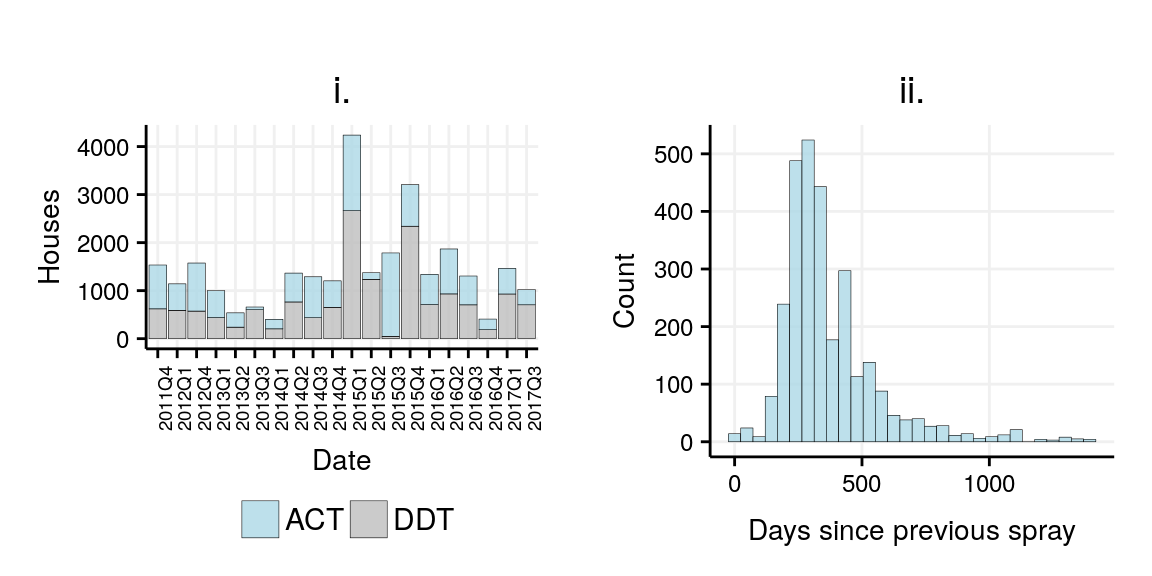
\includegraphics{sep2018_files/figure-latex/unnamed-chunk-7-1} \end{center}

\begin{center}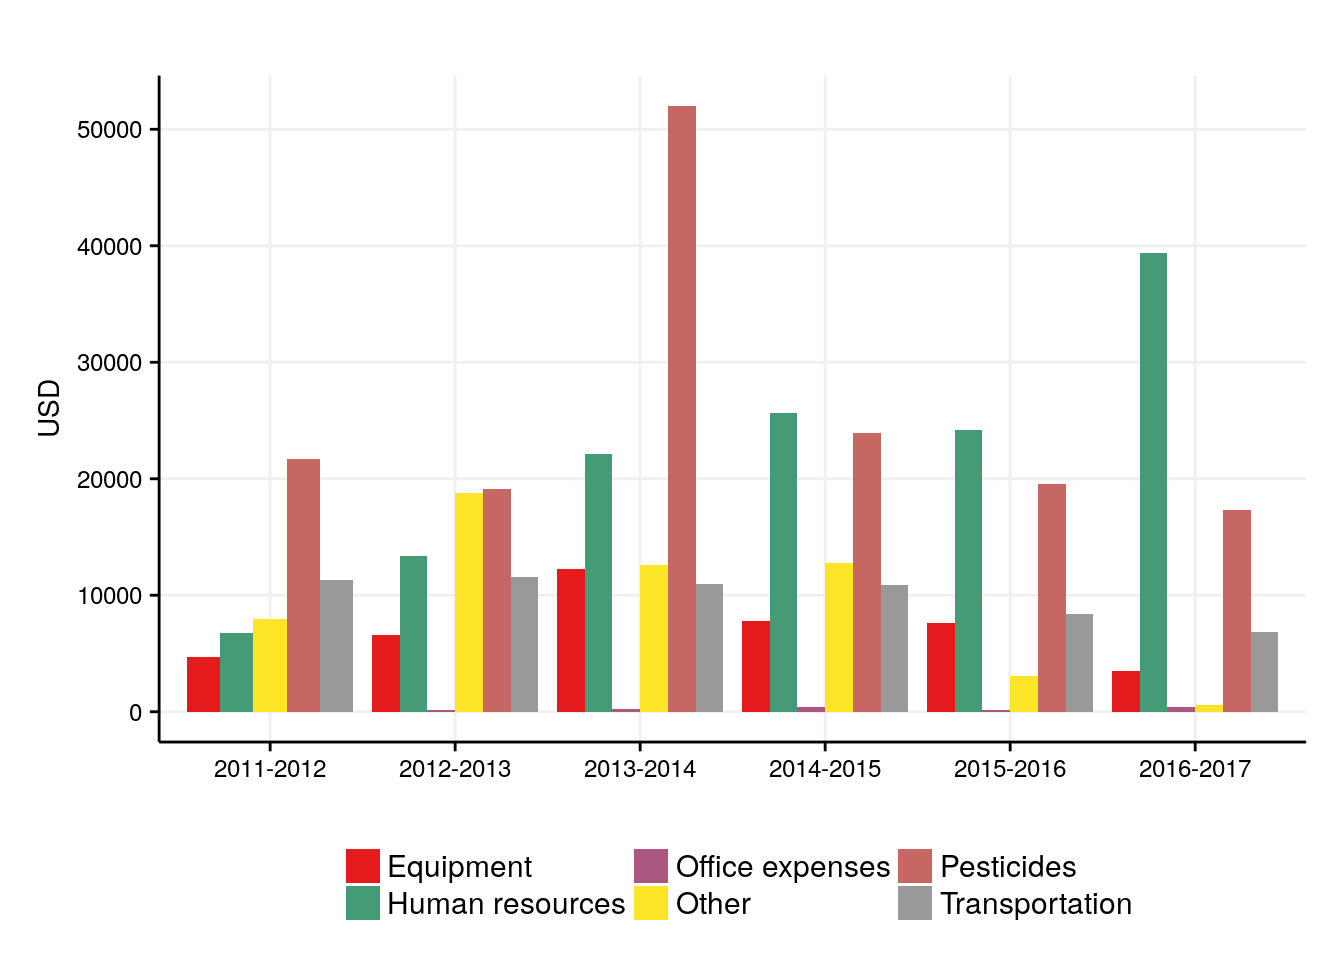
\includegraphics{sep2018_files/figure-latex/unnamed-chunk-8-1} \end{center}

\begin{center}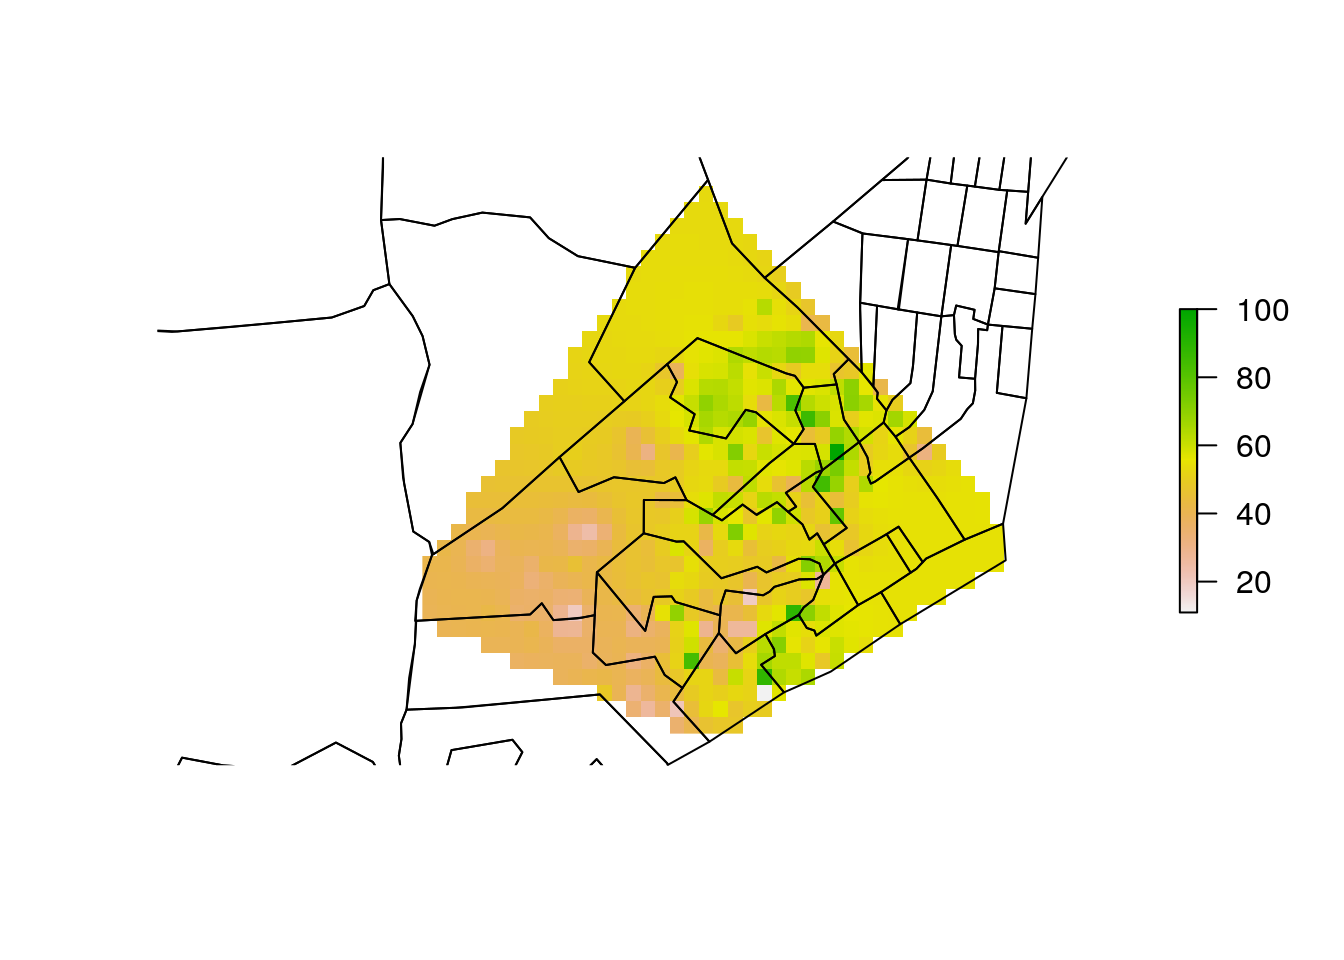
\includegraphics{sep2018_files/figure-latex/unnamed-chunk-9-1} \end{center}

\newpage

\subsection{Results}\label{results}

The below table shows the results of the model devised thus far.

\begin{longtable}[t]{ll}
\caption{\label{tab:unnamed-chunk-10}Model results}\\
\toprule
Term & Estimate\\
\midrule
protection & -0.192 (P=0.021)\\
Precipitation (mm) \_lag1\_3 & 0.04 (P=0.027)\\
\bottomrule
\end{longtable}

\subsection{Intepretation}\label{intepretation}

The below charts show predicted absenteeism rates at different rain and
protection levels.

\subsubsection{Precipitation's effect}\label{precipitations-effect}

\begin{center}\includegraphics{sep2018_files/figure-latex/unnamed-chunk-12-1} \end{center}

\subsubsection{IRS protection's effect}\label{irs-protections-effect}

\begin{center}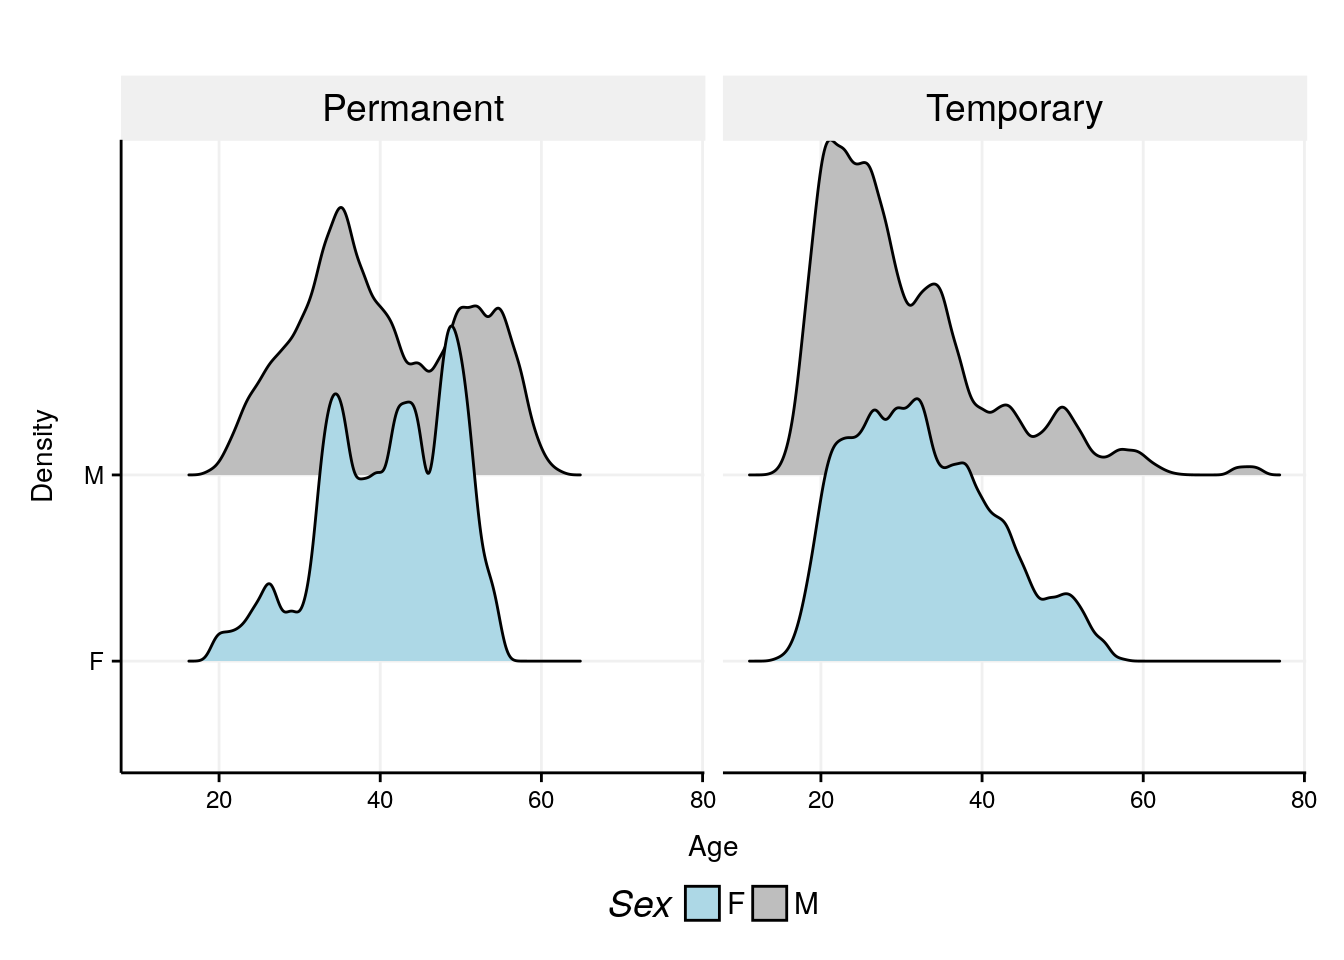
\includegraphics{sep2018_files/figure-latex/unnamed-chunk-13-1} \end{center}

\section*{Bibliography}\label{bibliography}
\addcontentsline{toc}{section}{Bibliography}

\hypertarget{refs}{}
\hypertarget{ref-Wu_2017}{}
Wu, Yunyun, Zhijiao Qiao, Nan Wang, Hongjie Yu, Zijian Feng, Xiaosong
Li, and Xing Zhao. 2017. ``Describing Interaction Effect Between Lagged
Rainfalls on Malaria: An Epidemiological Study in South--West China.''
\emph{Malaria Journal} 16 (1). Springer Nature.
doi:\href{https://doi.org/10.1186/s12936-017-1706-2}{10.1186/s12936-017-1706-2}.


\end{document}
